\begin{frame}[c]
	\frametitle{Facilitating higher-order approximation}
	\begin{itemize}\addtolength{\itemsep}{-.25\baselineskip}
	\item \alert{Hierarchical shape functions}
			\begin{itemize}
     		\item	\textit{\ltb{vertex functions}} supported by elements sharing the same vertex
     		\item<2-> \alert<2>{$p\geq 2$:} \textit{\ltb{edge functions}} supported by elems. sharing the same edge
     		\item<3-> \alert<3>{$p\geq 4$:} \textit{\ltb{bubble functions}} supported by a single element
			\end{itemize}
	\end{itemize}
	\only<1-3>{
	\begin{figure}\centering
		\only<1>{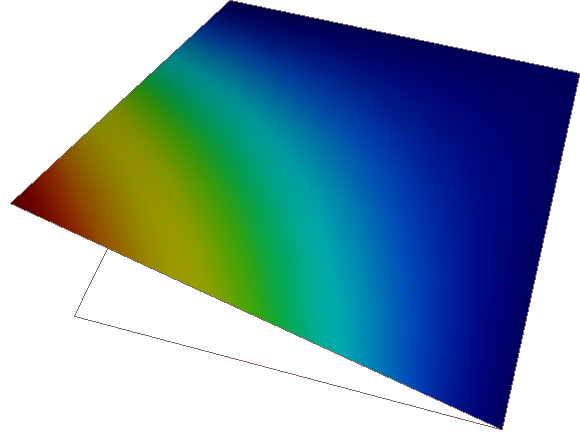
\includegraphics[scale=.3]{images/hsp/vtx}}
		\only<2>{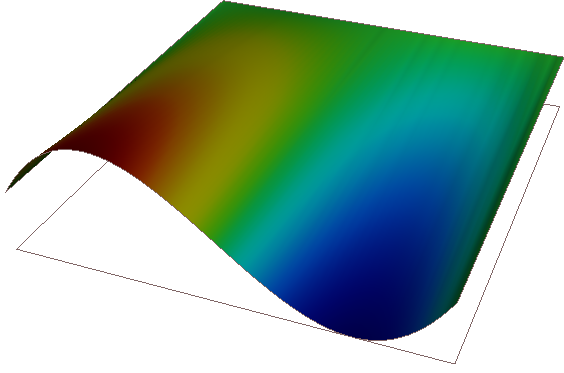
\includegraphics[scale=.3]{images/hsp/face}}
		\only<3>{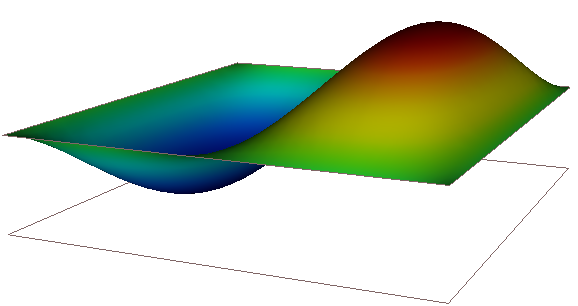
\includegraphics[scale=.3]{images/hsp/bubble}}
	\end{figure}
	}\vspace*{-1em}
	\begin{itemize}\addtolength{\itemsep}{-.25\baselineskip}
			\item<4-> $\mathrm{span}\, V^g_{h,p} \subset \mathrm{span}\, V^g_{h,p+1}$
			\item<5-> modifications req. when constraints appear due to hanging nodes 	  	
	\end{itemize}
\end{frame}
